\documentclass[tikz, border=2pt]{standalone}
\usepackage{tikz}
\usetikzlibrary{arrows.meta,positioning,fit,backgrounds,calc}
% Shared TikZ style, color-matched to paper/figures/*.pdf (matplotlib):
% ink = near-black strokes/fill, accent = deep red for the one thing per
% diagram that should draw the eye, grid = light gray for structure that
% should recede.
\definecolor{ink}{HTML}{1A1A1A}
\definecolor{accent}{HTML}{A6192E}
\definecolor{gridgray}{HTML}{D9D9D9}
\definecolor{panelbg}{HTML}{F2F2F2}

\tikzset{
  every node/.style={font=\sffamily},
  box/.style={draw=ink, thick, rounded corners=1.5pt, minimum height=0.75cm,
              font=\sffamily\small, align=center, fill=white, text=ink},
  stubbox/.style={box, draw=ink, dashed, fill=panelbg},
  hibox/.style={box, fill=ink, text=white},
  panel/.style={draw=none, fill=panelbg, rounded corners=2pt},
  arr/.style={-{Latex[length=2.2mm, width=1.6mm]}, thick, draw=ink},
  darr/.style={arr, dashed},
  accarr/.style={-{Latex[length=2.2mm, width=1.6mm]}, thick, draw=accent},
  lbl/.style={font=\sffamily\scriptsize, text=ink},
  ital/.style={font=\sffamily\itshape\scriptsize, text=ink!70},
  note/.style={font=\sffamily\scriptsize, align=left, text=ink},
  state/.style={draw=ink, thick, rounded corners=3pt, minimum width=2.6cm,
                minimum height=0.9cm, font=\sffamily\small, align=center, fill=white},
  finalstate/.style={state, fill=ink, text=white},
  abortstate/.style={state, draw=accent, thick, text=accent},
}

\begin{document}
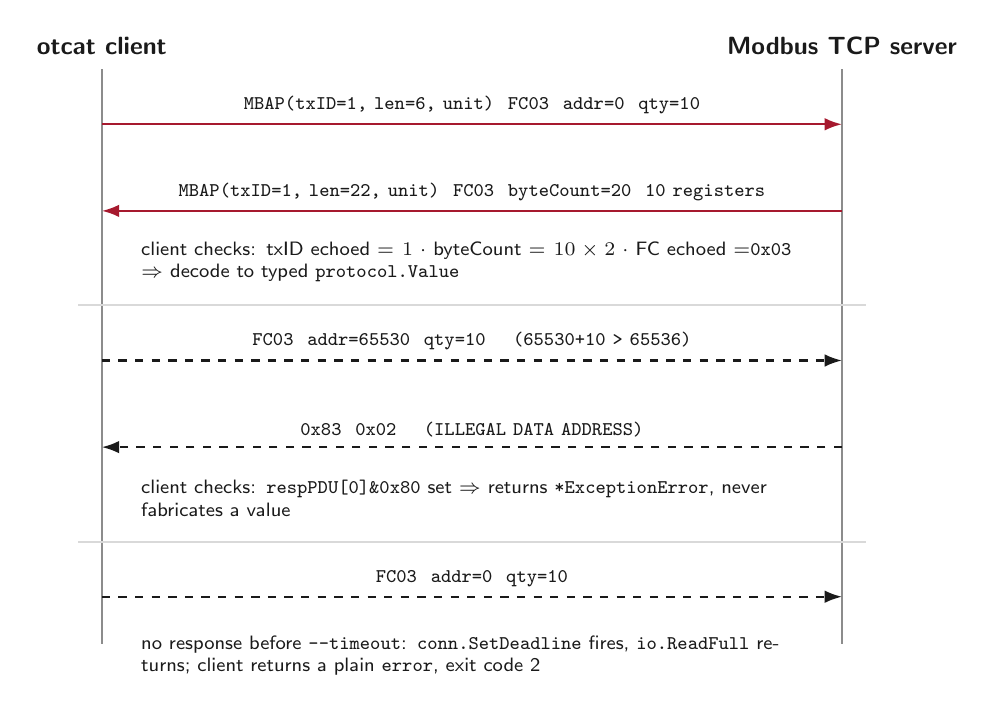
\begin{tikzpicture}

\node[lbl, font=\sffamily\bfseries\small] (C) at (0,7.6) {otcat client};
\node[lbl, font=\sffamily\bfseries\small] (S) at (9.4,7.6) {Modbus TCP server};
\draw[draw=ink!50, thick] (0,7.3) -- (0,0);
\draw[draw=ink!50, thick] (9.4,7.3) -- (9.4,0);

% --- happy path ---
\draw[accarr] (0,6.6) -- node[above, note, text width=8.6cm, align=center]
  {\ttfamily\scriptsize MBAP(txID=1, len=6, unit) \ FC03 \ addr=0 \ qty=10} (9.4,6.6);
\draw[accarr] (9.4,5.5) -- node[above, note, text width=8.6cm, align=center]
  {\ttfamily\scriptsize MBAP(txID=1, len=22, unit) \ FC03 \ byteCount=20 \ 10 registers} (0,5.5);
\node[note, text width=8.4cm] at (4.7,4.85)
  {client checks: txID echoed \(=1\) \(\cdot\) byteCount \(= 10\times2\) \(\cdot\) FC echoed \(=\)\texttt{0x03} \(\Rightarrow\) decode to typed \texttt{protocol.Value}};

\draw[draw=gridgray, thick] (-0.3,4.3) -- (9.7,4.3);

% --- exception path ---
\draw[darr] (0,3.6) -- node[above, note, text width=8.6cm, align=center]
  {\ttfamily\scriptsize FC03 \ addr=65530 \ qty=10 \quad(65530{+}10 > 65536)} (9.4,3.6);
\draw[darr] (9.4,2.5) -- node[above, note, text width=8.6cm, align=center]
  {\ttfamily\scriptsize 0x83 \ 0x02 \quad(ILLEGAL DATA ADDRESS)} (0,2.5);
\node[note, text width=8.4cm] at (4.7,1.85)
  {client checks: \texttt{respPDU[0]\&0x80} set \(\Rightarrow\) returns \texttt{*ExceptionError}, never fabricates a value};

\draw[draw=gridgray, thick] (-0.3,1.3) -- (9.7,1.3);

% --- timeout path ---
\draw[darr] (0,0.6) -- node[above, note, text width=8.6cm, align=center]
  {\ttfamily\scriptsize FC03 \ addr=0 \ qty=10} (9.4,0.6);
\node[note, text width=8.4cm] at (4.7,-0.15)
  {no response before \texttt{--timeout}: \texttt{conn.SetDeadline} fires, \texttt{io.ReadFull} returns; client returns a plain \texttt{error}, exit code 2};

\end{tikzpicture}
\end{document}
